\subsection{Power breakdown}

		\begin{table}[htb!]
			\centering
			\def\arraystretch{1.5}		
			\setlength\arrayrulewidth{0.75pt}
			\setlength{\tabcolsep}{1em} % for the horizontal padding
			\begin{tabular}{|c|c|c|c|c|}
				\hline 
				\rule[-1ex]{0pt}{2.5ex} \cellcolor{gray!40}\textbf{VCO} & \cellcolor{gray!40}\textbf{BBPD} & \cellcolor{gray!40}\textbf{Digital}& \cellcolor{gray!40}\textbf{CDACs} & \cellcolor{gray!40}\textbf{SUM} \\ 
				\hline 
				\rule[-1ex]{0pt}{2.5ex} 79.06 $\mu$W& 3.47 $\mu$W &  X $\mu$W  & X $ \mu$W & $\leq$ 100  $\mu$W\\ 
				\hline 
			\end{tabular} 
			\caption{Power breakdown.}
			\label{tab:power_bkdn}
		\end{table}   

		% \begin{table}[htb!]
		% 	\centering
		% 	\def\arraystretch{1.5}		
		% 	\setlength\arrayrulewidth{0.75pt}
		% 	\setlength{\tabcolsep}{1em} % for the horizontal padding
		% 	\begin{tabular}{|c|c|c|}
		% 		\hline 
		% 		\rule[-1ex]{0pt}{2.5ex} \cellcolor{gray!40}\textbf{Component} & \cellcolor{gray!40}\textbf{Power [$\mu$W]} & \cellcolor{gray!40}\textbf{\% of Total}\\ 
		% 		\hline 
		% 		\rule[-1ex]{0pt}{2.5ex} \textbf{VCO} &  227.8 & 4.5  \\ 
		% 		\hline 
		% 		\rule[-1ex]{0pt}{2.5ex} \textbf{2x 3b CDAC} &  735.0 &  14.4  \\ 
		% 		\hline 
		% 		\rule[-1ex]{0pt}{2.5ex} \textbf{2x 10b CDAC} &  1607.7 &  31.5  \\ 
		% 		\hline 
		% 		\rule[-1ex]{0pt}{2.5ex} \textbf{BBPD} &  5.31 &  0.1  \\ 
		% 		\hline 
		% 		\rule[-1ex]{0pt}{2.5ex} \textbf{Logic} &  1800 &  35.3  \\ 
		% 		\hline 
		% 		\rule[-1ex]{0pt}{2.5ex} \textbf{Other} &  724.2 &  14.2  \\ 
		% 		\hline 
		% 		\rule[-1ex]{0pt}{2.5ex} \textbf{Total} &  5100 &  100  \\ 
		% 		\hline 
		% 	\end{tabular} 
		% 	\caption{Power breakdown.}
		% 	\label{tab:power_bkdn}
		% \end{table}   


		\begin{figure}[htb!]
	        \centering
	        \includegraphics[width=0.65\textwidth, angle=0]{example-image}
		    \caption{PLL Power breakdown.}
		    \label{fig:pow_bkdn}
		\end{figure}

\subsection{Area Breakdown}
The implemented area is 60 $\mu$m $\times$ 85 $\mu$m, or 0.0051 mm$^2$. The breakdown of the implemented area is in table \ref{tab:area_bkdn}.

		\begin{table}[htb!]
			\centering
			\def\arraystretch{1.5}		
			\setlength\arrayrulewidth{0.75pt}
			\setlength{\tabcolsep}{1em} % for the horizontal padding
			\begin{tabular}{|c|c|c|}
				\hline 
				\rule[-1ex]{0pt}{2.5ex} \cellcolor{gray!40}\textbf{Component} & \cellcolor{gray!40}\textbf{Area [$\mu$m$^2$]} & \cellcolor{gray!40}\textbf{\% of Total}\\ 
				\hline 
				\rule[-1ex]{0pt}{2.5ex} \textbf{VCO} &  227.8 & 4.5  \\ 
				\hline 
				\rule[-1ex]{0pt}{2.5ex} \textbf{2x 3b CDAC} &  735.0 &  14.4  \\ 
				\hline 
				\rule[-1ex]{0pt}{2.5ex} \textbf{2x 10b CDAC} &  1607.7 &  31.5  \\ 
				\hline 
				\rule[-1ex]{0pt}{2.5ex} \textbf{BBPD} &  5.31 &  0.1  \\ 
				\hline 
				\rule[-1ex]{0pt}{2.5ex} \textbf{Logic} &  1800 &  35.3  \\ 
				\hline 
				\rule[-1ex]{0pt}{2.5ex} \textbf{Other} &  724.2 &  14.2  \\ 
				\hline 
				\rule[-1ex]{0pt}{2.5ex} \textbf{Total} &  5100 &  100  \\ 
				\hline 
			\end{tabular} 
			\caption{Area breakdown.}
			\label{tab:area_bkdn}
		\end{table}   


\subsection{Phase Noise}
	\hl{Bandwidth and integrated phase noise power values.}
		\begin{figure}[htb!]
	        \centering
	        \includegraphics[width=0.65\textwidth, angle=0]{example-image}
		    \caption{PLL phase noise SSB spectral density.}
		    \label{fig:sim_pll_psd}
		\end{figure}

\subsection{Start-up Transient}
	\hl{Lock time value.}
		\begin{figure}[htb!]
	        \centering
	        \includegraphics[width=0.65\textwidth, angle=0]{example-image}
		    \caption{PLL start up transient.}
		    \label{fig:sim_pll_trans}
		\end{figure}
{\color{white}.}

\FloatBarrier\pagebreak
\subsection{Voltage Controlled Oscillator}\label{sec:ro_results}

		\begin{table}[htb!]
			\centering
			\def\arraystretch{1.5}		
			\setlength\arrayrulewidth{0.75pt}
			\setlength{\tabcolsep}{1em} % for the horizontal padding
			\begin{tabular}{|c|c|c|}
				\hline 
				\rule[-1ex]{0pt}{2.5ex} \cellcolor{gray!40}\textbf{Parameter} & \cellcolor{gray!40}\textbf{Value} & \cellcolor{gray!40}\textbf{Units}\\ 
				\hline 
				\rule[-1ex]{0pt}{2.5ex} \textbf{FOM$_{pn}$} & -157.2 & dB  \\ 
				\hline 
				\rule[-1ex]{0pt}{2.5ex} $S_{0_{osc}}$ &  11885 &  rad$^2$/Hz  \\ 
				\hline 
				\rule[-1ex]{0pt}{2.5ex} \textbf{Power} &  79.06 &  $\mu$W  \\ 
				\hline 
				\rule[-1ex]{0pt}{2.5ex} \textbf{RMS Frequency Variance} &  34.5 / 4.2 &  MHz / \%  \\ 
				\hline 
			\end{tabular} 
			\caption{Ring oscillator performance parameters.}
			\label{tab:ro_perf}
		\end{table}   

	\subsubsection{Phase Noise}
		\begin{figure}[htb!]
	        \centering
	        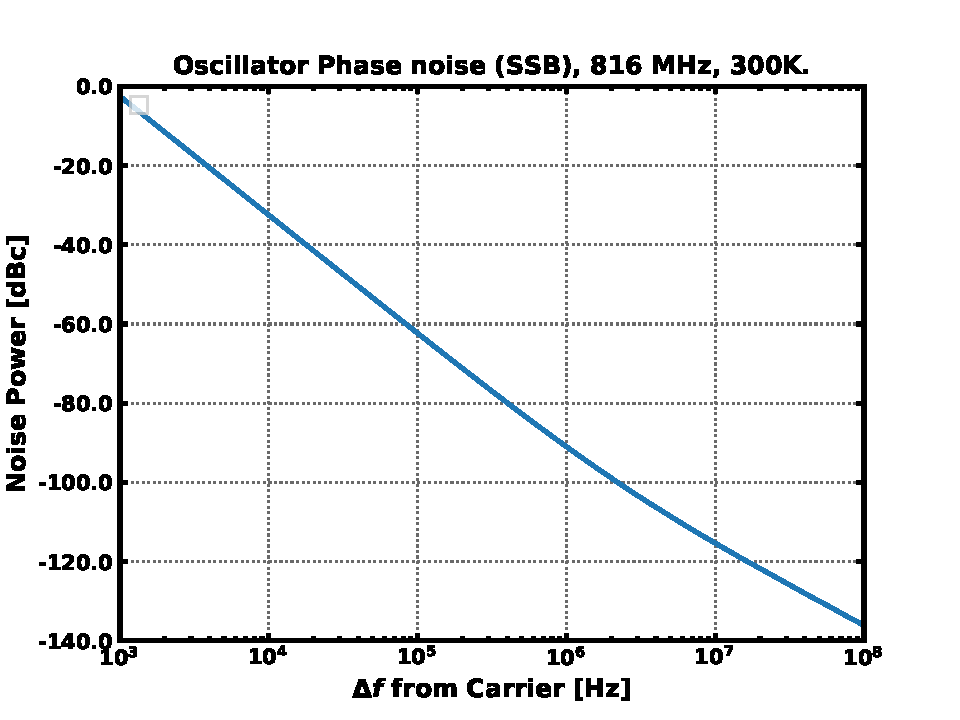
\includegraphics[width=0.55\textwidth, angle=0]{./figs/results/osc_pnoise}
		    \caption{Ring oscillator phase noise (SSB).}
		    \label{fig:ro_pnoise}
		\end{figure}
	\FloatBarrier

	\subsubsection{Frequency}
		\begin{figure}[htb!]
	        \centering
	        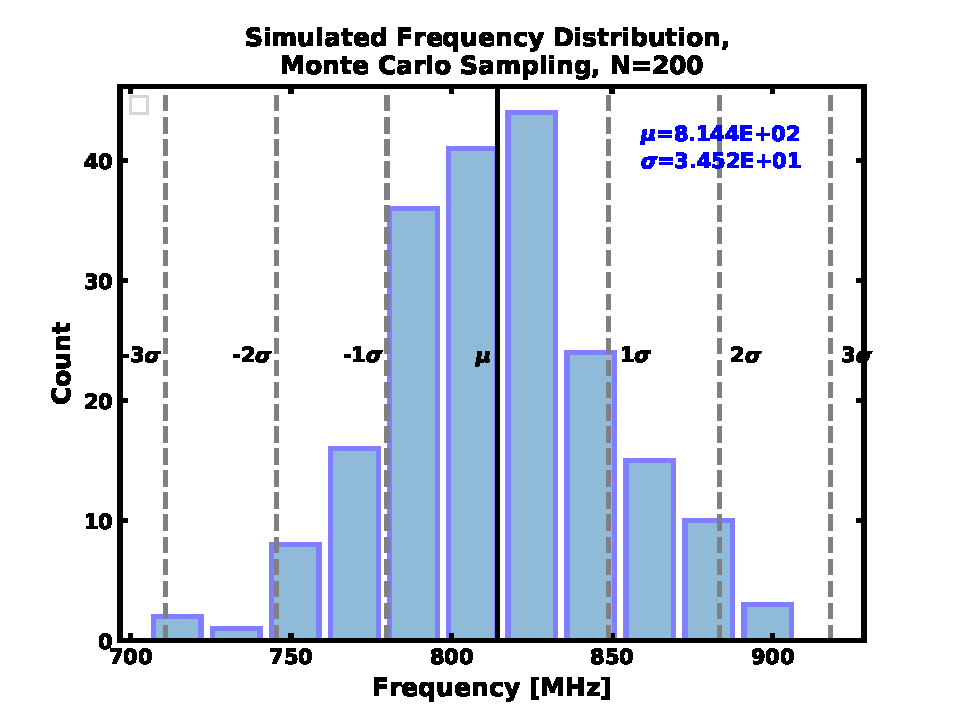
\includegraphics[width=0.55\textwidth, angle=0]{./figs/results/freq_pdf}
		    \caption{Variation of oscillator frequency from Monte-Carlo variation/mismatch simulation.}
		    \label{fig:freq_variation}
		\end{figure}
	\FloatBarrier
	\subsubsection{Tuning}
		\begin{table}[h!]
			\centering
			\def\arraystretch{1.5}		
			\setlength\arrayrulewidth{0.75pt}
			\setlength{\tabcolsep}{1em} % for the horizontal padding
			\begin{tabular}{|l|r|l|r|l|}
				\hline 
				\rule[-1ex]{0pt}{2.5ex} \cellcolor{gray!40}\textbf{Mode} & \cellcolor{gray!40}\textbf{VCO Gain} & \cellcolor{gray!40}\textbf{Units} & \cellcolor{gray!40}\textbf{Normalized gain}& \cellcolor{gray!40}\textbf{Units}\\ 
				\hline 
				\rule[-1ex]{0pt}{2.5ex} \textbf{Supply tuning}  & 2.588 & MHz/mV & 317.2 &\%/V\\
				\hline 
				\rule[-1ex]{0pt}{2.5ex} \textbf{Medium tuning}  & 30.92 & kHz/mV  & 3.789 &\%/V\\
				\hline 
				\rule[-1ex]{0pt}{2.5ex} \textbf{Fine tuning}  & 5.378 & kHz/mV & 0.659 & \%/V\\
				\hline 
				\rule[-1ex]{0pt}{2.5ex} \textbf{Capacitor tuning} & 9782 & kHz/cap & 1.19 & \%/cap\\
				\hline 
			\end{tabular} 
			% \caption{Assigned specifications for branch line hybrid design.}
			% \label{asgn_specs}
			\caption{PLL parameters determined from filter design and optimization process for fast lock speed with TDC feedback.}
			\label{tab:vco_gains}
		\end{table} 

	\begin{figure}[htb!]
	    \centering
	    \begin{subfigure}{0.5\textwidth}
	        \centering
	        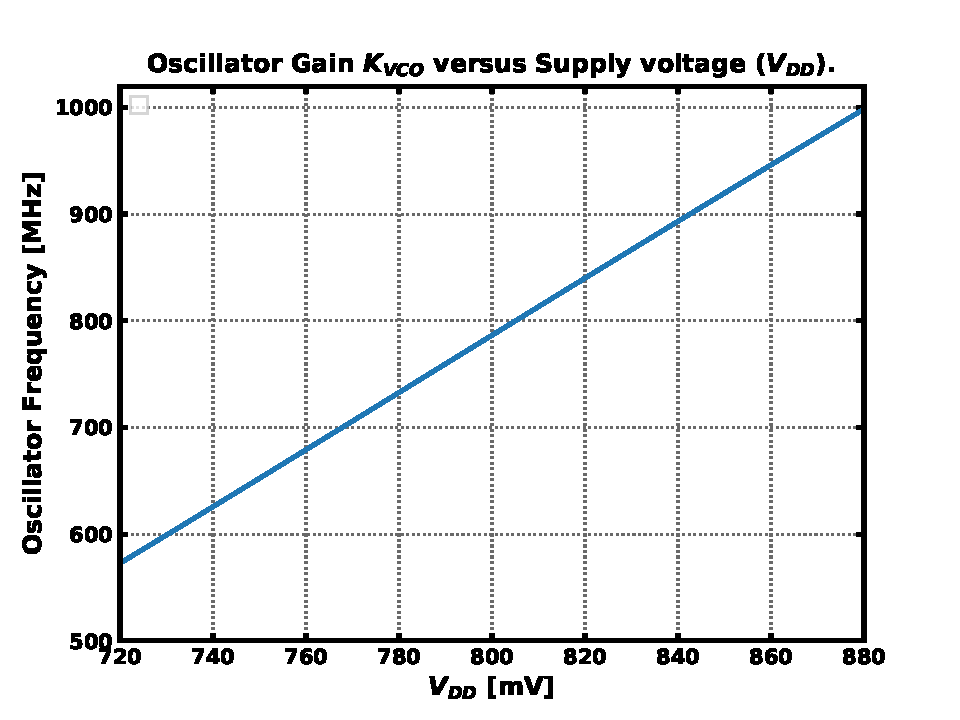
\includegraphics[width=1\textwidth, angle=0]{./figs/results/osc_f_vs_vdd}
	        \caption{ }
	        \label{fig:osc_f_vs_vdd}
	    \end{subfigure}%
	    \begin{subfigure}{0.5\textwidth}
	        \centering
	        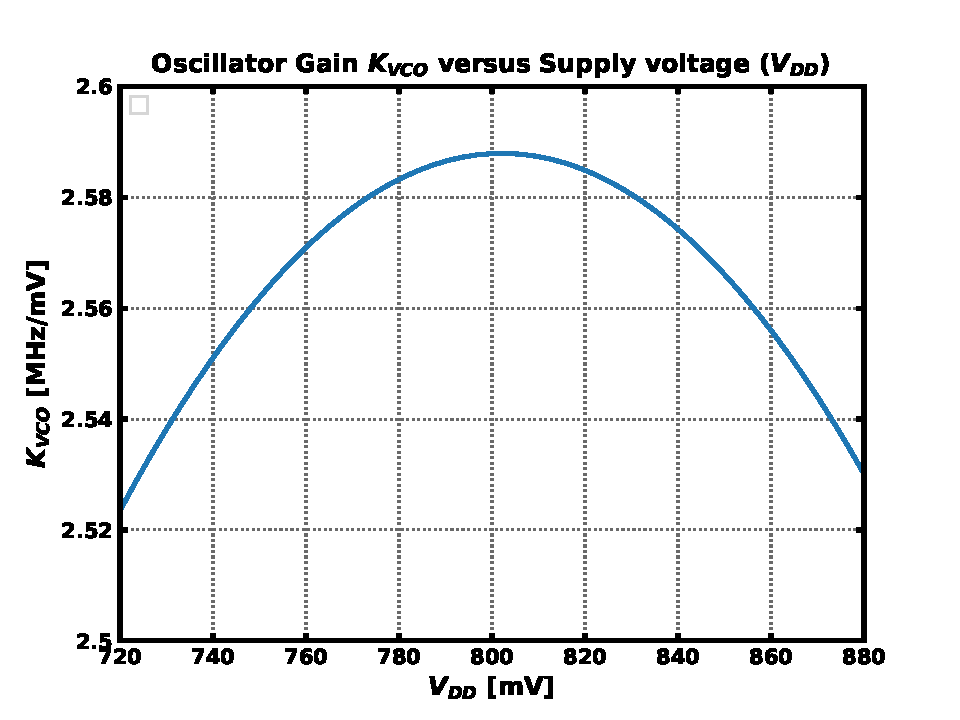
\includegraphics[width=1\textwidth, angle=0]{./figs/results/osc_f_gain_vs_vdd}
	        \caption{ }
	        \label{fig:osc_f_gain_vs_vdd}
	    \end{subfigure}
	    % \caption{x.}
	    \label{fig:osc_f_vdd}
	    \caption{Supply voltage versus ($\pm$ 10\% from 0.8V) \textbf{(a)} Oscillation Frequency, \textbf{(b)} VCO gain.}
	\end{figure} 

	\begin{figure}[htb!]
	    \centering
	    \begin{subfigure}{0.5\textwidth}
	        \centering
	        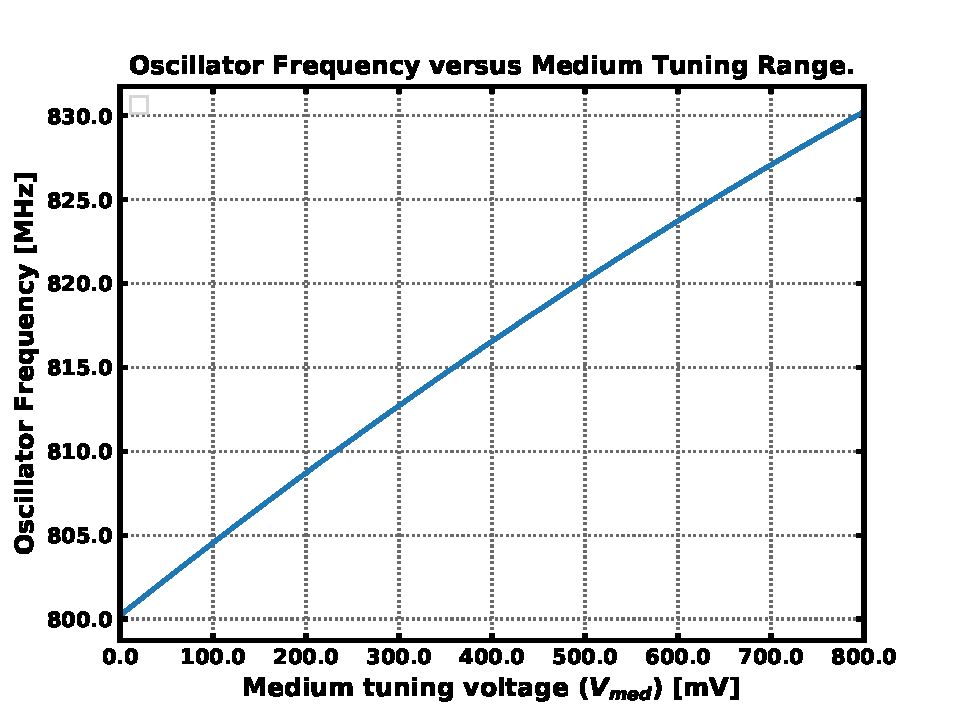
\includegraphics[width=1\textwidth, angle=0]{./figs/results/osc_f_vs_med}
	        \caption{ }
	        \label{fig:osc_f_vs_med}
	    \end{subfigure}%
	    \begin{subfigure}{0.5\textwidth}
	        \centering
	        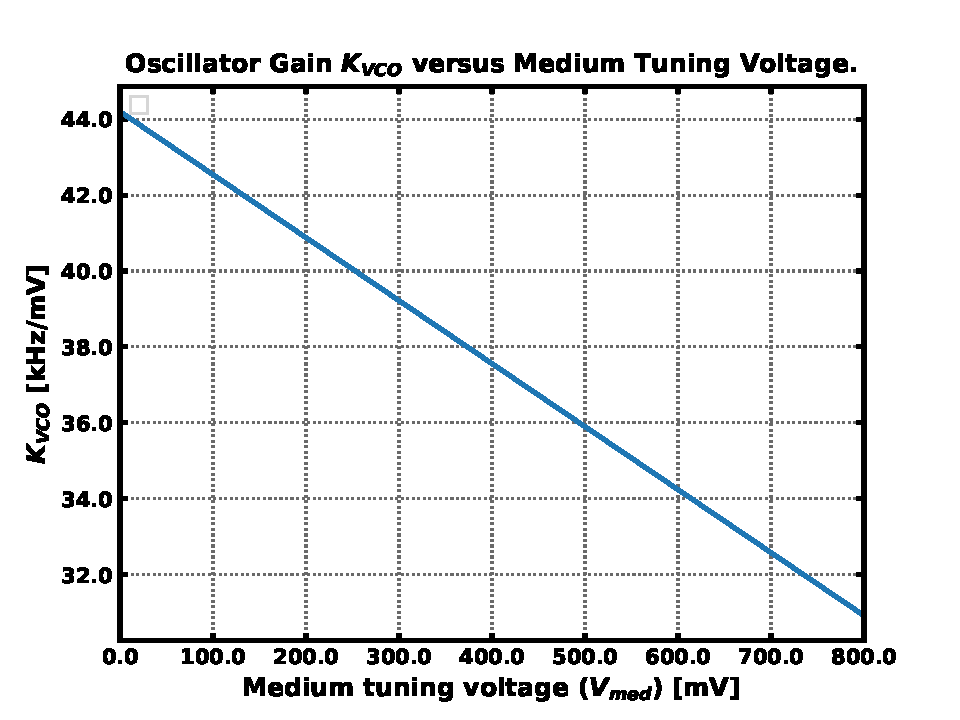
\includegraphics[width=1\textwidth, angle=0]{./figs/results/osc_f_gain_vs_med}
	        \caption{ }
	        \label{fig:osc_f_gain_vs_med}
	    \end{subfigure}
	    % \caption{x.}
	    \label{fig:osc_f_med_tune}
	    \caption{Medium tuning range versus \textbf{(a)} Oscillation Frequency, \textbf{(b)} VCO gain.}
	\end{figure} 


	\begin{figure}[htb!]
	    \centering
	    \begin{subfigure}{0.5\textwidth}
	        \centering
	        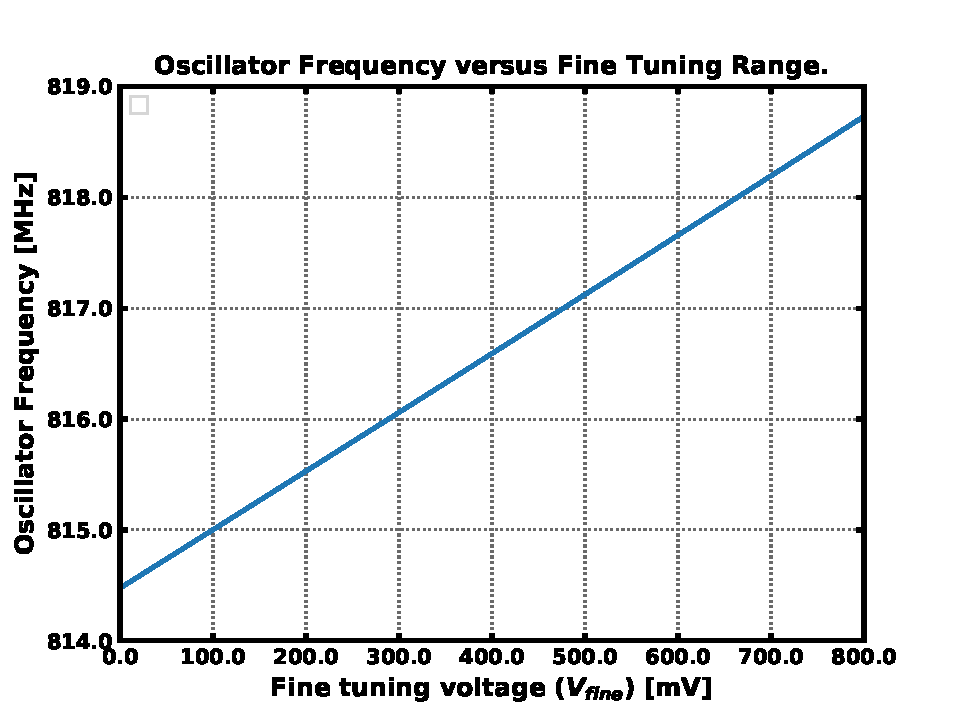
\includegraphics[width=1\textwidth, angle=0]{./figs/results/osc_f_vs_fine}
	        \caption{ }
	        \label{fig:osc_f_vs_fine}
	    \end{subfigure}%
	    \begin{subfigure}{0.5\textwidth}
	        \centering
	        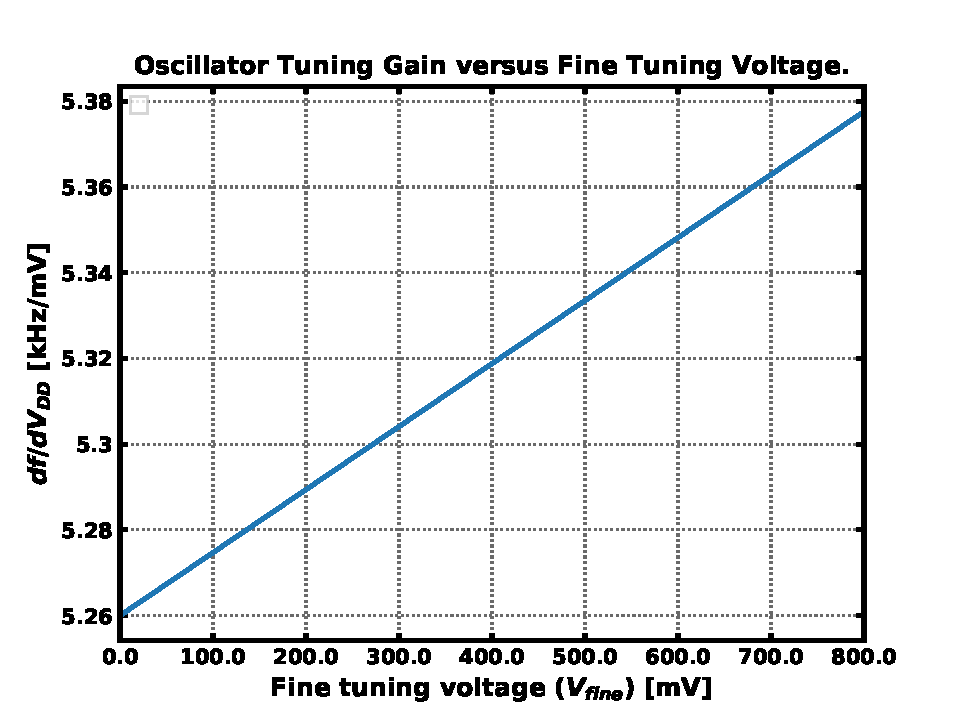
\includegraphics[width=1\textwidth, angle=0]{./figs/results/osc_f_gain_vs_fine}
	        \caption{ }
	        \label{fig:osc_f_gain_vs_fine}
	    \end{subfigure}
	    % \caption{x.}
	    \label{fig:osc_f_fine_tune}
	    \caption{Fine tuning range versus \textbf{(a)} Oscillation Frequency, \textbf{(b)} VCO gain.}
	\end{figure} 



		\begin{figure}[htb!]
	        \centering
	        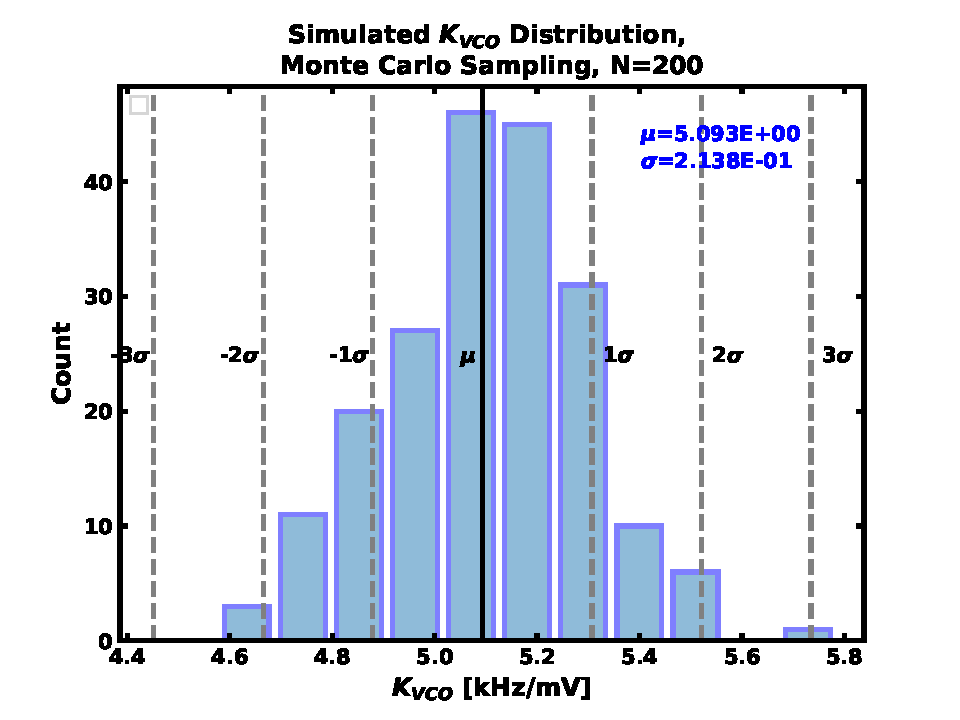
\includegraphics[width=0.5\textwidth, angle=0]{./figs/results/kvco_pdf}
		    \caption{Variation of VCO fine tuning gain from Monte-Carlo variation/mismatch simulation.}
		    \label{fig:kvco_variation}
		\end{figure}

	\FloatBarrier
	\subsubsection{Waveforms}
			\begin{figure}[htb!]
			    \centering
			    \begin{subfigure}{0.5\textwidth}
			        \centering
			        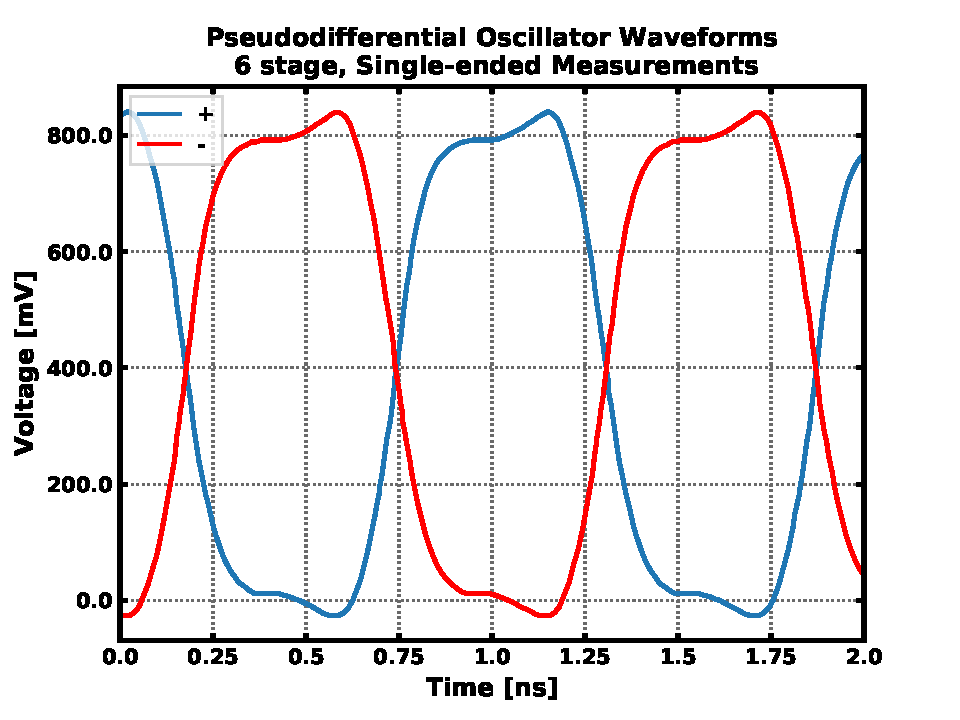
\includegraphics[width=1\textwidth, angle=0]{./figs/results/osc_se_waves}
			        \caption{ }
			        \label{fig:osc_se_waves}
			    \end{subfigure}%
			    \begin{subfigure}{0.5\textwidth}
			        \centering
			        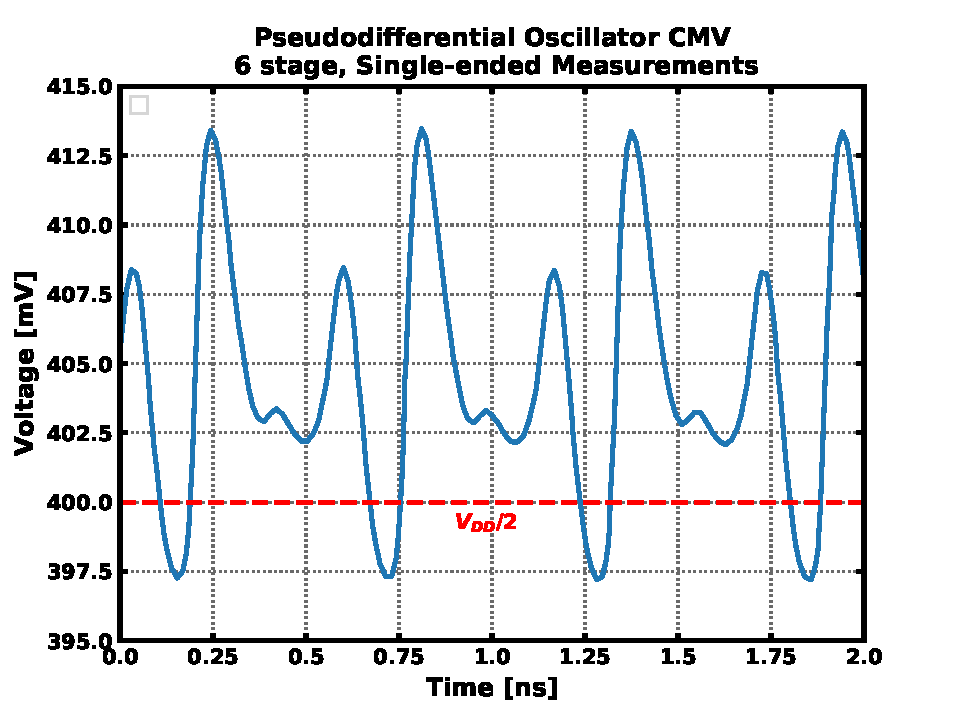
\includegraphics[width=1\textwidth, angle=0]{./figs/results/osc_cmv}
			        \caption{ }
			        \label{fig:osc_cmv}
			    \end{subfigure}
			    % \caption{x.}
			    \label{fig:osc_waves}
			    \caption{\textbf{(a)} Oscillator single-ended waveforms, \textbf{(b)} Oscillator common mode voltage waveform.}
			\end{figure} 
	\FloatBarrier
\FloatBarrier
\subsection{10b CDAC}\label{sec:res_cdac_10b}

	\begin{figure}[htb!]
	    \centering
	    \begin{subfigure}{0.5\textwidth}
	        \centering
	        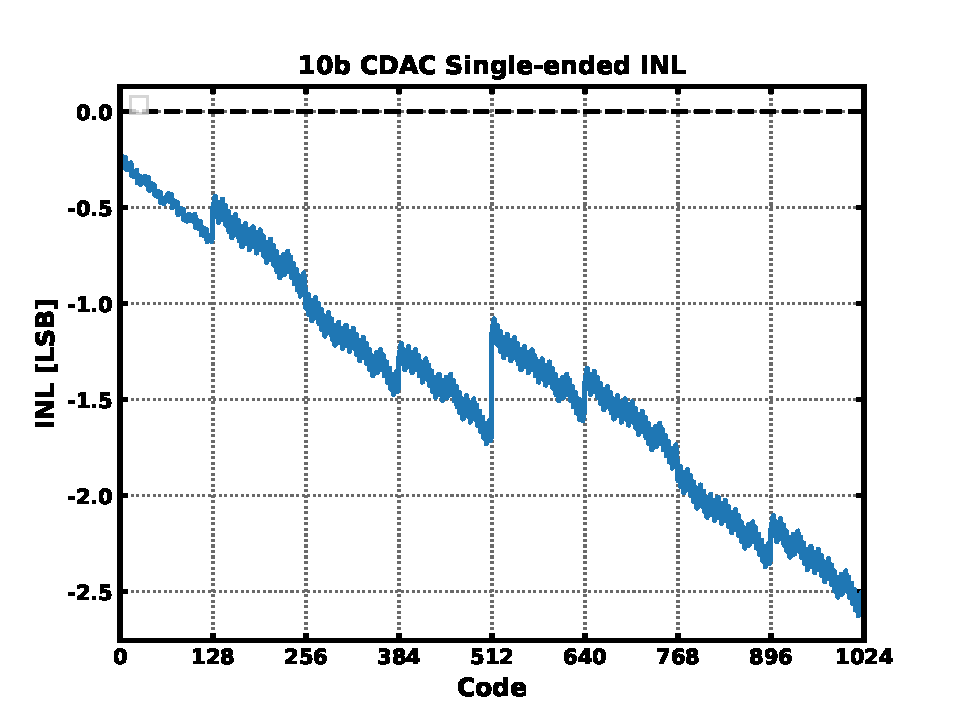
\includegraphics[width=1\textwidth, angle=0]{./figs/results/10b_cdac_se_inl}
	        \caption{ }
	        \label{fig:10b_cdac_se_inl}
	    \end{subfigure}%
	    \begin{subfigure}{0.5\textwidth}
	        \centering
	        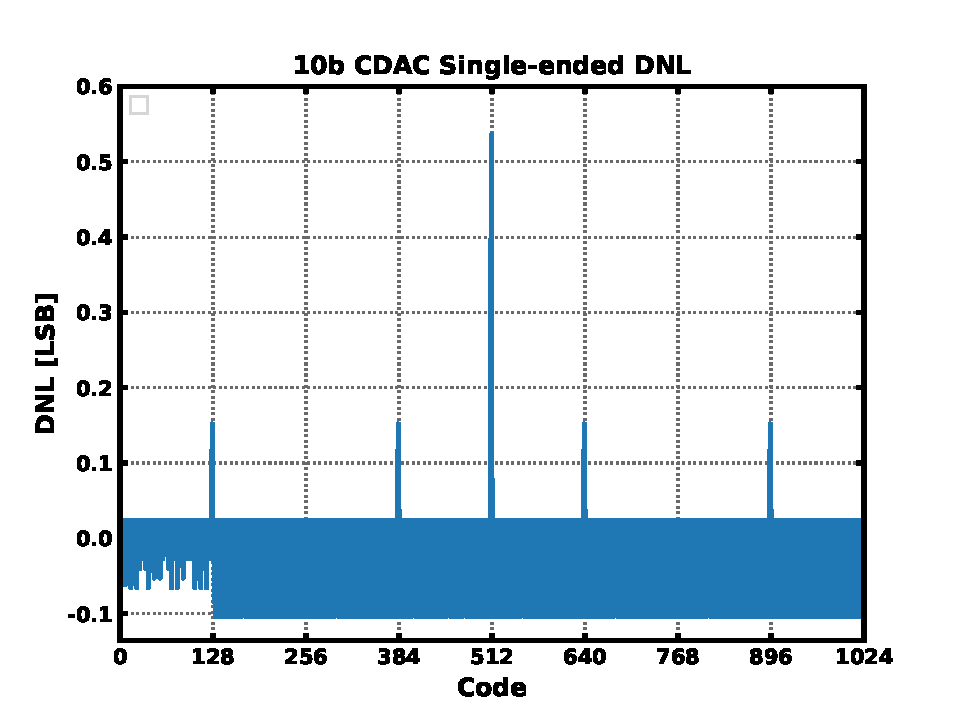
\includegraphics[width=1\textwidth, angle=0]{./figs/results/10b_cdac_se_dnl}
	        \caption{ }
	        \label{fig:10b_cdac_se_dnl}
	    \end{subfigure}
	    % \caption{x.}
	    \label{fig:10b_cdac_se_nonlinearity}
	    \caption{10b CDAC single-ended \textbf{(a)} Integral Nonlinearity, \textbf{(b)} Differential Nonlinearity.}
	\end{figure} 



	\begin{figure}[htb!]
	    \centering
	    \begin{subfigure}{0.5\textwidth}
	        \centering
	        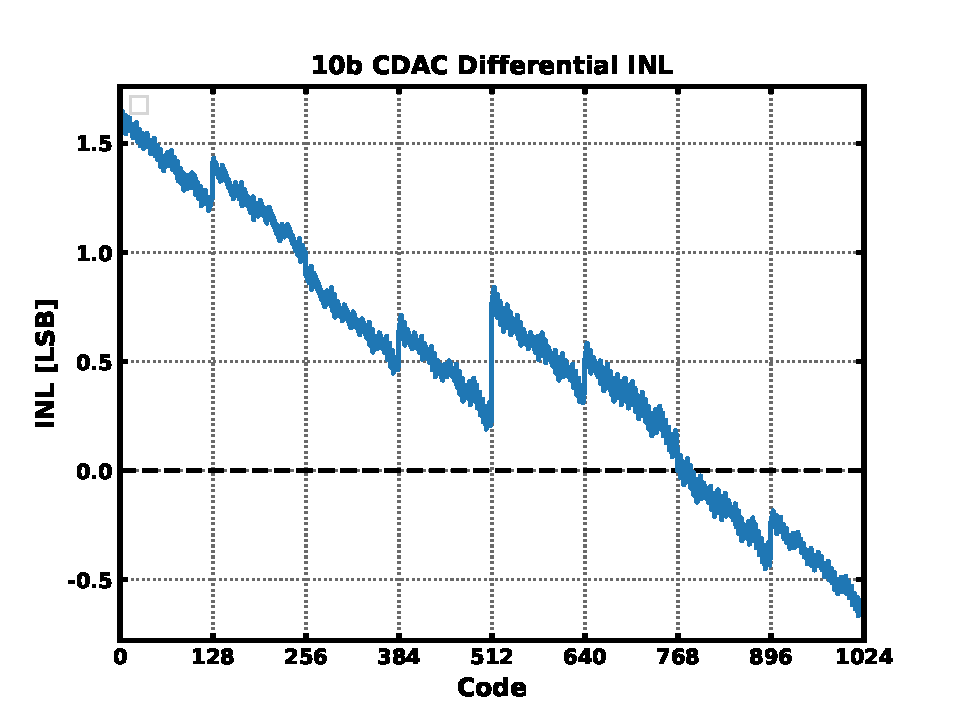
\includegraphics[width=1\textwidth, angle=0]{./figs/results/10b_cdac_diff_inl}
	        \caption{ }
	        \label{fig:10b_cdac_diff_inl}
	    \end{subfigure}%
	    \begin{subfigure}{0.5\textwidth}
	        \centering
	        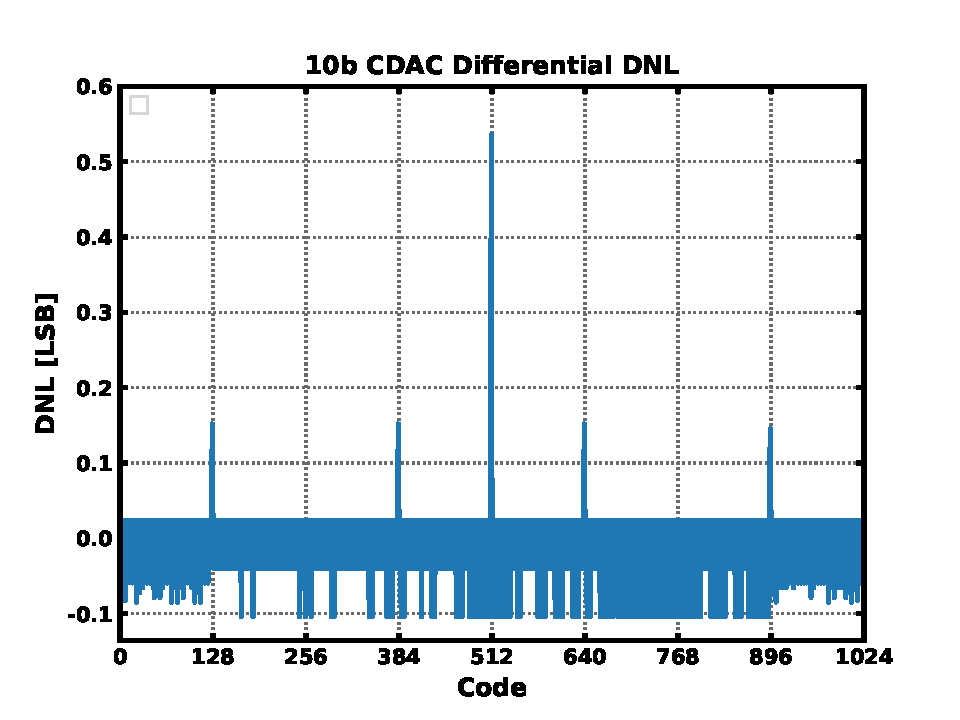
\includegraphics[width=1\textwidth, angle=0]{./figs/results/10b_cdac_diff_dnl}
	        \caption{ }
	        \label{fig:10b_cdac_diff_dnl}
	    \end{subfigure}
	    % \caption{x.}
	    \label{fig:10b_cdac_diff_nonlinearity}
	    \caption{10b CDAC differential \textbf{(a)} Integral Nonlinearity, \textbf{(b)} Differential Nonlinearity.}
	\end{figure} 


\FloatBarrier\pagebreak
\subsection{3b CDAC}\label{sec:res_cdac_3b}

	\begin{figure}[htb!]
	    \centering
	    \begin{subfigure}{0.5\textwidth}
	        \centering
	        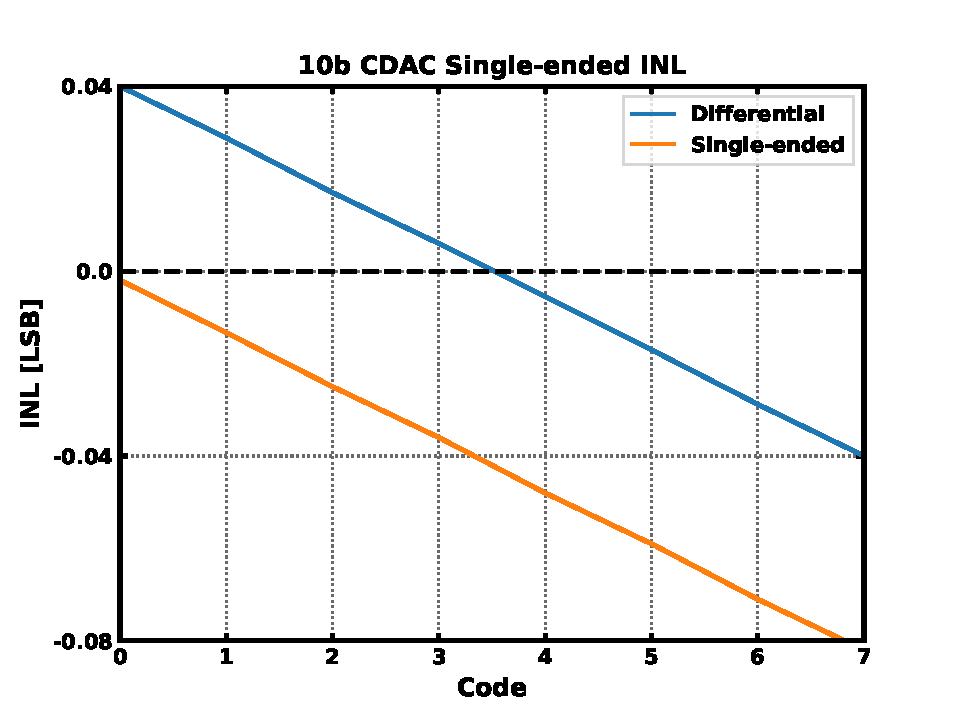
\includegraphics[width=1\textwidth, angle=0]{./figs/results/cdac_3b_inl}
	        \caption{ }
	        \label{fig:cdac_3b_inl}
	    \end{subfigure}%
	    \begin{subfigure}{0.5\textwidth}
	        \centering
	        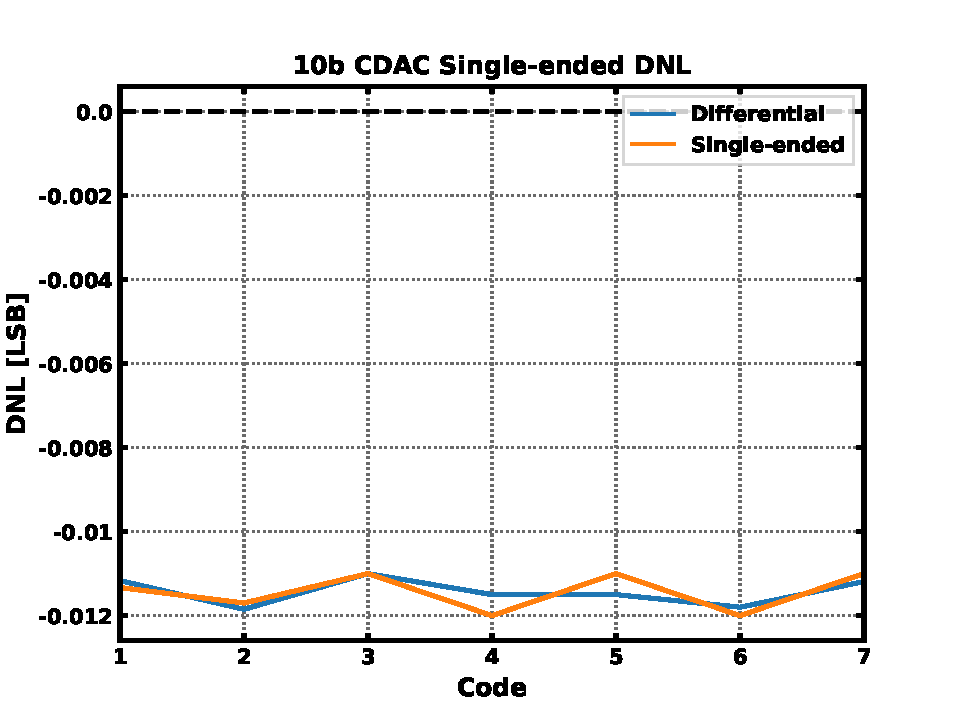
\includegraphics[width=1\textwidth, angle=0]{./figs/results/cdac_3b_dnl}
	        \caption{ }
	        \label{fig:cdac_3b_dnl}
	    \end{subfigure}
	    % \caption{x.}
	    \label{fig:3b_cdac_nonlinearity}
	    \caption{3b CDAC differential \textbf{(a)} Integral Nonlinearity, \textbf{(b)} Differential Nonlinearity.}
	\end{figure} 


\FloatBarrier
\subsection{Bang-bang phase detector}\label{sec:res_bbpd}
With noise simulated up to 20 GHz, the RMS jitter of the detector is 1.342ps.

	\begin{figure}[htb!]
	    \centering
	    \begin{subfigure}{0.5\textwidth}
	        \centering
	        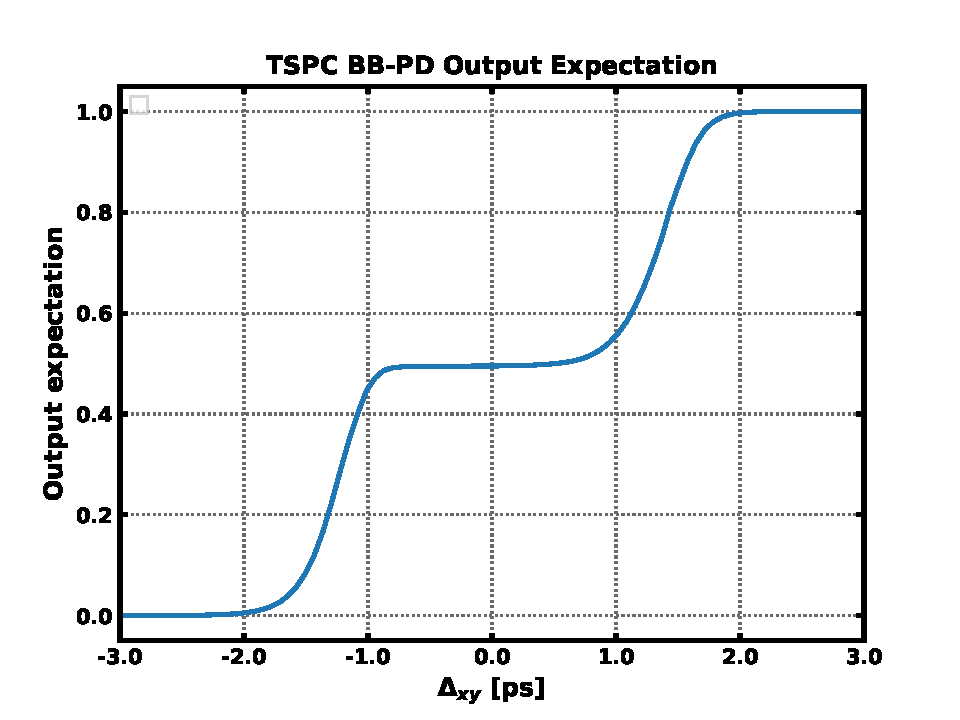
\includegraphics[width=1\textwidth, angle=0]{./figs/results/cdf}
	        \caption{ }
	        \label{fig:bbpd_cdf}
	    \end{subfigure}%
	    \begin{subfigure}{0.5\textwidth}
	        \centering
	        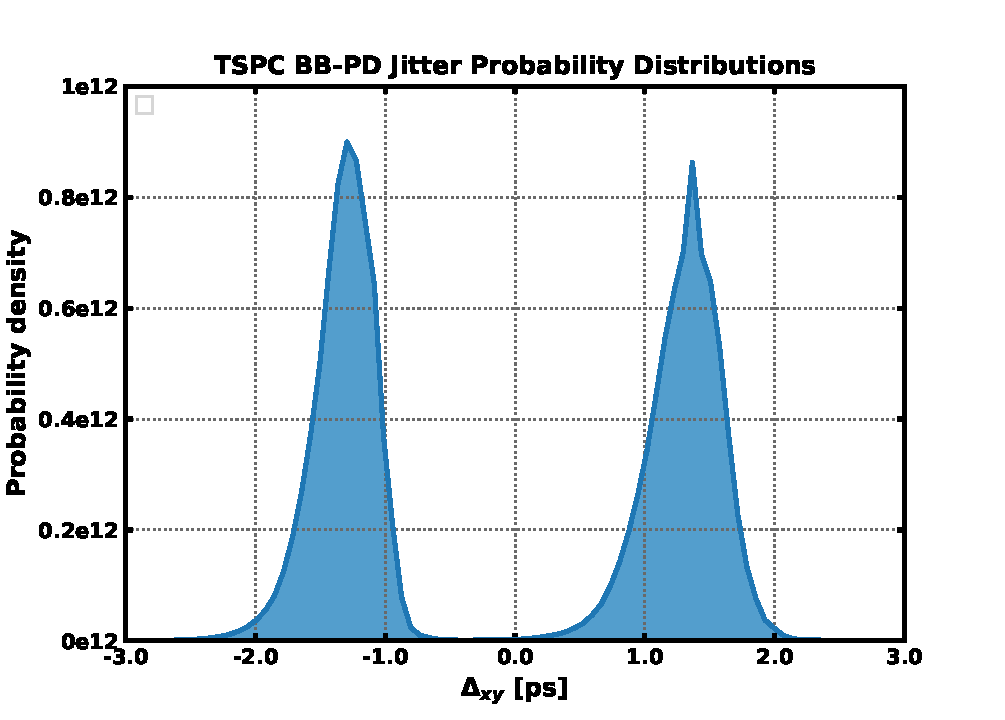
\includegraphics[width=1\textwidth, angle=0]{./figs/results/pdf}
	        \caption{ }
	        \label{fig:bbpd_pdf}
	    \end{subfigure}
	    % \caption{x.}
	    \label{fig:bbpd_jitter_dist}
	    \caption{BBPD extracted jitter \textbf{(a)} Cumulative Distribution Function, \textbf{(b)} Probability Distribution Function.}
	\end{figure} 

\FloatBarrier\pagebreak
\subsection{Loop filter }\label{sec:rec_lf}
	\subsubsection{Optimal Paramters}
		\begin{table}[h!]
			\centering
			\def\arraystretch{1.5}		
			\setlength\arrayrulewidth{0.75pt}
			\setlength{\tabcolsep}{1em} % for the horizontal padding
			\begin{tabular}{|l|r|l|}
				\hline 
				\rule[-1ex]{0pt}{2.5ex} \cellcolor{gray!40}\textbf{Parameter} & \cellcolor{gray!40}\textbf{Value} & \cellcolor{gray!40}\textbf{Unit }\\ 
				\hline 
				\rule[-1ex]{0pt}{2.5ex} \textbf{$K$}  & $1.6400055\times10^{15}$ &  \\
				\hline 
				\rule[-1ex]{0pt}{2.5ex} \textbf{$K_i$}  & $3.904893\times10^{11}$ &  \\
				\hline 
				\rule[-1ex]{0pt}{2.5ex} \textbf{$K_p$}  & $1.928457\times10^4$ &  \\
				\hline 
				\rule[-1ex]{0pt}{2.5ex} \textbf{$f_z$} & $3.222697\times10^5$ & Hz\\
				\hline 
				\rule[-1ex]{0pt}{2.5ex} \textbf{$b_0$}  & $4.369015\times10^4$  &\\
				\hline 
				\rule[-1ex]{0pt}{2.5ex} \textbf{$b_1$}  & $-1.92845\times10^4$  & \\
				\hline 
				\rule[-1ex]{0pt}{2.5ex} Estimated bandwidth & $1.6\times10^6$ & Hz \\
				\hline 
				\rule[-1ex]{0pt}{2.5ex} Estimated lock time & $9.65873\times10^{-7}$ & seconds \\
				\hline 
			\end{tabular} 
			% \caption{Assigned specifications for branch line hybrid design.}
			% \label{asgn_specs}
			\caption{PLL parameters determined from filter design and optimization process for fast lock speed with synchronous counter feedback.}
			\label{filter_params_fast_lock}
		\end{table}   

		\begin{table}[h!]
			\centering
			\def\arraystretch{1.5}		
			\setlength\arrayrulewidth{0.75pt}
			\setlength{\tabcolsep}{1em} % for the horizontal padding
			\begin{tabular}{|l|r|l|}
				\hline 
				\rule[-1ex]{0pt}{2.5ex} \cellcolor{gray!40}\textbf{Parameter} & \cellcolor{gray!40}\textbf{Value} & \cellcolor{gray!40}\textbf{Unit }\\ 
				\hline 
				\rule[-1ex]{0pt}{2.5ex} \textbf{$K$}  & $9.64757\times12^{12}$ &  \\
				\hline 
				\rule[-1ex]{0pt}{2.5ex} \textbf{$K_i$}  & $2.991366\times10^{7}$ &  \\
				\hline 
				\rule[-1ex]{0pt}{2.5ex} \textbf{$K_p$}  & $1.926152\times10^{1}$ &  \\
				\hline 
				\rule[-1ex]{0pt}{2.5ex} \textbf{$f_z$} & $0.494343\times10^5$ & Hz\\
				\hline 
				\rule[-1ex]{0pt}{2.5ex} \textbf{$b_0$}  & $2.300073\times10^1$  &\\
				\hline 
				\rule[-1ex]{0pt}{2.5ex} \textbf{$b_1$}  & $-1.926152\times10^1$  & \\
				\hline 
				\rule[-1ex]{0pt}{2.5ex} Estimated bandwidth & $1.227156\times10^6$ & Hz \\
				\hline 
				\rule[-1ex]{0pt}{2.5ex} Estimated lock time & $9.65873\times10^{-7}$ & seconds \\
				\hline 
			\end{tabular} 
			% \caption{Assigned specifications for branch line hybrid design.}
			% \label{asgn_specs}
			\caption{PLL parameters determined from filter design and optimization process for minimum phase noise with BBPD.}
			\label{filter_params_bbpd_low_noise}
		\end{table}   
		\subsubsection{Digital Implementation Parameters}
		\begin{table}[h!]
			\centering
			\def\arraystretch{1.5}		
			\setlength\arrayrulewidth{0.75pt}
			\setlength{\tabcolsep}{1em} % for the horizontal padding
			\begin{tabular}{|l|r|r|l|}
				\hline 
				\rule[-1ex]{0pt}{2.5ex} \cellcolor{gray!40}\textbf{Parameter} & \cellcolor{gray!40}\textbf{Value} & \cellcolor{gray!40}\textbf{Value (digital) } & \cellcolor{gray!40}\textbf{Value Error}\\ 
				\hline 
				\rule[-1ex]{0pt}{2.5ex} Total dataword bits  & 16 & & \\ 
				\hline 
				\rule[-1ex]{0pt}{2.5ex} Sign bits  & 1 & & \\ 
				\hline 
				\rule[-1ex]{0pt}{2.5ex} Integer bits & 4 & & \\ 
				\hline 
				\rule[-1ex]{0pt}{2.5ex} Fractional bits  & 11 & & \\ 
				\hline 
				\rule[-1ex]{0pt}{2.5ex} \textbf{$b_0$} {\color{red} (gear 1)} & $2.301440\times10^2$ & \texttt{0bX}  & $+x\times10^{-x}$\\
				\hline 
				\rule[-1ex]{0pt}{2.5ex} \textbf{$b_1$} {\color{red} (gear 1)} & $-2.115054\times10^2$ & \texttt{0bX}  & $+x\times10^{-x}$\\
				\hline 
				\rule[-1ex]{0pt}{2.5ex} \textbf{$b_0$} {\color{blue} (gear 2)} & $2.300073\times10^1$ & \texttt{0bX}  & $+x\times10^{-x}$ \\
				\hline 
				\rule[-1ex]{0pt}{2.5ex} \textbf{$b_1$} {\color{blue} (gear 2)} & $-1.926152\times10^1$ & \texttt{0bX}  & $+x\times10^{-x}$\\
				\hline 
			\end{tabular} 
			% \caption{Assigned specifications for branch line hybrid design.}
			% \label{asgn_specs}
			\caption{Loop filter digitized coefficients.}
			\label{dig_filter_params_fast}
		\end{table}  

\FloatBarrier\subsection{Logic}

		\begin{table}[htb!]
			\centering
			\def\arraystretch{1.5}		
			\setlength\arrayrulewidth{0.75pt}
			\setlength{\tabcolsep}{1em} % for the horizontal padding
			\begin{tabular}{|c|c|c|c|}
				\hline 
				\rule[-1ex]{0pt}{2.5ex} \cellcolor{gray!40}\textbf{Component} & \cellcolor{gray!40}\textbf{Count } & \cellcolor{gray!40}\textbf{Area [$\mu$m$^2$]}& \cellcolor{gray!40}\textbf{Area (\% total)}\\ 
				\hline 
				\rule[-1ex]{0pt}{2.5ex} \textbf{Sequential (DFF)} &  210 & 228.8 & 31.9 \\ 
				\hline 
				\rule[-1ex]{0pt}{2.5ex} \textbf{Inverter} & 112 & 14.9 & 2.1  \\ 
				\hline 
				\rule[-1ex]{0pt}{2.5ex} \textbf{Logic Gates} & 684 & 472.9 & 66.0  \\ 
				\hline 
				\rule[-1ex]{0pt}{2.5ex} \textbf{Total} & 1006 & 716.9 & 100  \\ 
				\hline 
			\end{tabular} 
			\caption{Synthesisized logic counts.}
			\label{tab:log_synth}
		\end{table}   


% \FloatBarrier\subsection{Synchronous counter}
% Power consumption